bb\section{Analisa}
  
    \subsection{Analisa Paper Rujukan}
    Dengan perkembangan teknologi, perlahan kebiasaan manusia berubah. Termasuk juga dalam perdagangan, dimana transaksi jual beli barang tidak lagi harus melalui tatap muka. Penjualan online saat ini sudah dapat dilakukan lewat berbagai cara, antara lain menggunakan e-commerce, atau posting di social media, atau bisa juga dengan melelang di aplikasi lelang online. Sedikit berbeda dengan teknik penjualan di lelang online, karena aplikasi ini dapat diakses oleh banyak orang, tentu saja pelelang (auctioneer) tidak terbatas pada ruang lelang saja, tapi bisa berasal dari manapun selama mereka mengakses aplikasi tersebut.  Lelang online ini tentu saja mendatangkan banyak manfaat, selain biaya yang lebih efisien dan hemat, dan juga tidak menguras waktu karena siapapun, kapanpun, dimanapun dapat mengajukan penawaran ataupun melelang barangnya tanpa harus pergi ke instansi tertentu dan melakukan lelang dengan cara konvensional.
    Bercermin terhadap aplikasi \textit{e-commerce} yang telah ada, masalah yang paling sering dialami adalah ketidakpuasan pengguna. Salah satu indikator bahwa suatu perusahaan dikatakan memiliki ketidakpuasan pelanggan adalah karena kegagalan dalam pelayanannya. Seorang pelanggan sangat mungkin memutuskan untuk komplain setelah mengalami ketidakpuasan terhadap layanan suatu perusahaan, dan jika tidak ditangani dengan baik, hal ini bisa berakibat fatal terhadap reputasi dan kepercayaan pengguna terhadap aplikasi tersebut.
    Oleh karena itu, sebuah paper mengangkat topik ini khusus dalam bidang aplikasi lelang online, menganalisa kegagalan dan ketidakpuasan pengguna, beserta solusi-solusi yang ditawarkan oleh pengguna aplikasi untuk memperbaiki kegagalan pelayanan tersebut. 
	  \begin{figure}[H]
        \centering
        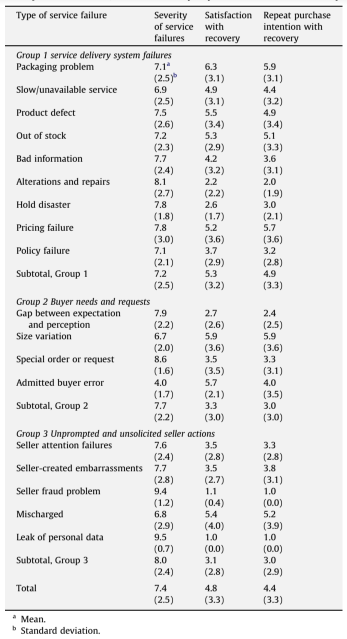
\includegraphics[width=\linewidth]{images/bab3/Fatalitas-Kegagalan-Ecommerce.png}
        \caption{Fatalitas kegagalan dalam aplikasi Lelang Online, Kepuasan terhadap Perbaikan Pelayanan dan \textit{Repeat Purchase Intention} setelah Perbaikan Layanan}
        \label{severity-failures}
      \end{figure}
      
      Dalam gambar diatas, dijabarkan beberapa jenis kegagalan yang pernah dialami oleh pengguna aplikasi serta fatalitas/pengaruh buruk kegagalan tersebut terhadap kepercayaan pengguna. 
      
	  \begin{figure}[H]
        \centering
        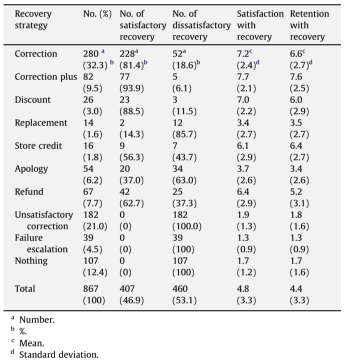
\includegraphics[width=\linewidth]{images/bab3/Solusi-Perbaikan-Ketidakpuasan.png}
        \caption{Kategori Perbaikan terhadap Kegagalan Pelayanan Lelang Online}
        \label{service-recovery-strategies}
      \end{figure}
      
      Dalam gambar diatas, dijabarkan beberapa solusi yang pernah ditawarkan kepada pengguna aplikasi serta kepuasan dan ketidakpuasan terhada solusi yang diberikan
      
      
`'      Maka berdasarkan hasil analisa tersebut, fitur-fitur yang perlu ditambahkan selain daripada fitur dasar aplikasi lelang online adalah sebagai berikut :
      \begin{enumerate}
      \item Fitur chatting, untuk mengurangi kemungkinan \textit{Bad Information} dimana ekspektasi dan persepsi terhadap barang yang dilelang antara pembeli dan penjual tidak sama dan \textit{Special Needs}, 
      \item Fitur pemberian kupon voucher (\textit{Discount and Correction Plus}) yang bisa berupa \textit{free shipping} atau \textit{discount}.
      \end{enumerate}
  
 
	\subsection{Analisa \textit{User Experience} dari E-Commerce di Indonesia}
    \label{alasan-ux-ecommerce-indonesia alasan-app-serupa}
    Pada saat awal pengerjaan dan pada masa pengerjaan juga, penulis sering sekali menganalisa dan memperhatikan kebiasaan-kebiasaan yang diciptakan saat sedang \textit{browsing} di website \textit{e-commerce} di Indonesia. Salah satu yang paling sering adalah Tokopedia.
    Beberapa hal yang saya perhatikan adalah :
    \begin{enumerate}
    \item Halaman yang muncul bukanlah eagerloading, tapi \textit{lazy loading} - dimana perlahan-lahan komponen muncul satu per satu, hingga semua komponen lengkap ditampilkan.
    \linebreak
    Ini adalah solusi cerdas untuk mengakali \textit{delay loading item} yang sudah pasti jumlahnya sangat banyak (maka butuh \textit{query} yang tentunya memakan waktu cukup lama), namun juga memainkan faktor psikologi / \textit{user behaviour} pengguna dengan membiarkan pengguna melihat tahap demi tahap halaman 'diisi'.
    \linebreak
    Saya pun mencoba menerapkan ini dalam aplikasi Lelang Online ini dengan menggunakan \textit{tools} Vue.js
    \item Layouting yang sederhana namun ringkas - adalah konsep dengan warna-warna yang juga sederhana, tidak terlalu kontras dan tidak terlalu halus untuk dilihat.
    \end{enumerate}
    Dari 2 poin tersebut, sebisa mungkin saya adaptasi ke dalam aplikasi Lelang Online ini.
    
    \subsection{Analisa Keamanan pada koneksi Soket}
    \label{alasan-socket.io}
    Untuk mengakomodasi fitur yang bersifat \textit{realtime}, dibutuhkan koneksi ke soket secara terus menerus. Hal ini tentu dapat menjadi sasaran empuk \textit{security} karena jika tidak diamankan, maka dapat menjadi peluang besar bagi para pihak yang tidak berkepentingan untuk merusak proses bisnis aplikasi.
    Namun, jika dalam setiap koneksi soket harus mengirimkan \textit{credentials}, hal ini tentu menjadi tidak praktis dan malah lebih berbahaya karena membiarkan data-data sensitif seperti \textit{password} dan \textit{username} berlalu-lalang di jaringan internet. Selain itu, \textit{disadvantage}nya adalah ketidakpraktisan untuk selalu meng\textit{query} database setiap kali ada koneksi, tentu saja ini memperlambat kerja \textit{database} dan menambah waktu \textit{delay}.
    Untuk menyiasatinya, penulis menerapkan JWT.io dengan keuntungan sebagai berikut :
    \begin{enumerate}
    \item Tidak perlu \textit{query} ke database karena hanya menggunakan security token yang di\textit{generate} dengan formula tertentu
    \item Tidak perlu ada aplikasi khusus yang menjembatani aplikasi Soket dan aplikasi WebServer - sehingga lebih praktis
    \item Data-data sensitif menjadi lebih terjaga karena tidak perlu dipertukarkan setiap koneksi ke soket.
    \end{enumerate}
    
    \subsection{Analisa \textit{Best Practice} dalam Struktur Perangkat Lunak}
    \label{alasan-best-practice}
    Pada dasarnya, Laravel adalah kerangka kerja MVC. Namun, ada banyak fitur yang ada dalam aplikasi Lelang Online ini yang tidak terakomodasi dalam MVC, misal sebagai berikut :
    \begin{enumerate}
    \item Sistem Verifikasi lewat Email - yang berarti aplikasi harus berinteraksi dengan SMTP server
    \item Sistem \textit{Generate} Token JWT.io , dimana dalam proses \textit{Generate Token} sama sekali tidak ada database dilibatkan.
    \end{enumerate}
    
    Jika fitur-fitur tersebut 'dipaksa' dimuat ke dalam MVC, maka tentu saja strukturnya menjadi ganjil, dan muncul \textit{code smell} berikut :
    \begin{enumerate}
    \item \textit{Large Class}, dimana terdapat satu buah file yang sangat panjang (biasanya merupakan entitas utama, dalam hal ini contohnya barang/\textit{item})
    \item \textit{Inappropriate Intimacy}, dimana terdapat satu kelas yang menyimpan \textit{logic} yang tidak seharusnya ia simpan
    \item \textit{Duplicated Code}
    \end{enumerate}
    
    Untuk menghindari kemungkinan \textit{code smell} tersebut, maka penulis menyiasatinya dengan cara berikut :
    \begin{enumerate}
    \item Penggunaan Repository Pattern untuk memisahkan antara Data Processing Layer dan View Layer.
    Selain lebih rapi, terstruktur, hal ini juga dapat menghindari \textit{Duplicated Code}.
    \item Penambahan komponen baru yaitu Service dan Provider, untuk memisahkan dan merapikan struktur aplikasi.
    Tujuannya, agar jika kedepannya terdapat perbaikan fitur/penambahan fitur, lebih mudah \textit{traceback} terhadap file/kelas yang bertanggungjawab terhadap fitur tersebut.
	\end{enumerate}
    
    \subsection{Analisa Aplikasi Serupa}
    \label{alasan-app-serupa}
    Selama penulisan dan pembuatan aplikasi, penulis selalu mencoba menganalisa aplikasi serupa. Dan pada akhirnya, penulis menemukan aplikasi yang kurang lebih alur bisnis / alur penggunaan aplikasinya serupa yaitu : Carousell.
	Penulis melihat ada beberapa kesamaan antara sifat transaksi aplikasi tugas akhir saya dengan aplikasi tersebut, yaitu :
	\begin{enumerate}
	\item Sama-sama tidak mengakomodasi pembayaran
    \item Sama-sama tidak adanya kepastian harga (bedanya, pada carousell.com yang terjadi adalah bargaining
	\end{enumerate}
	Jadi, untuk alur proses nya, banyak saya adaptasi dari Carousell, dengan maksud agar pengguna lebih familiar dan paham jika mengikuti \textit{base practice} di E-commerce lainnya yang lebih umum digunakan ole pengguna